%
% 
%
%%%%%%%%%%%%%%%%%%%%%%%%%%%%%%%%%%%%%%%%%%%%%%%%%%%%%%%%%%%%%%%%%%%%%%%%
\chapter{Recurrence Relation in CPPINTS}


%%%%%%%%%%%%%%%%%%%%%%%%%%%%%%%%%%%%%%%%%%%%%%%%%%%%%%%%%%%%%%%%%%%%%%%%
\section{Introduction to Analytical Integral Algorithms}
\label{concepts_introduction}

The integral we discussed here is analytical integrals,
which is generally expressed as:
\begin{equation}\label{int_paper:1}
  I_{ijkl} = \int \chi_{i}(\bm{r})\chi_{j}(\bm{r})f(\bm{r},\bm{r^{'}})
\chi_{k}(\bm{r^{'}})\chi_{l}(\bm{r^{'}}) d\bm{r} d\bm{r^{'}}
\end{equation}
and the integrand is analytically integrated. Kinetic integrals(KI),
nuclear attraction integrals(NAI), electron repulsion integrals(ERI) etc. all 
belong to this group. 

Since Boys\cite{SFBoys1950} suggested to use Cartesian Gaussian type function to form 
basis functions,
\begin{equation}\label{int_paper:2}
 \chi = x^{i}y^{j}z^{k}e^{-\alpha r^{2}}
\end{equation}
a major breakthrough technology for computing ERI was introduced by Pople and Hehre(PH)\cite{PH}. 
This method provides exceptional efficient algorithm for computing high contracted 
low angular momentum integrals. However, this method is limited to S and P basis functions, 
and it's difficult to be extended to high angular momentum integrals. McMurchie and 
Davidson(MD)\cite{MD}
proposed a general formalism for computing variety kind of analytical integrals in terms of 
Hermitian polynomials, and their method is applied to integrals with high angular momentum. 
Dupuis, Rys and King(DRK)\cite{DRK1976JCOMP,DRK1976JCP,DRK1983JCOMP} developed another formalism 
for ERI based on exact numerical 
quadrature using root and weights generated from Rys polynomials. Although MD and DRK
methods provide general way to derive the analytical integrals, they are indirect methods where
auxiliary polynomials need to be involved. 

In 1980s, Obara and Saika(OS)\cite{OS1986,OS1988} derived a set of
recursive formulas for analytical integrals based on recursive expression of 
three body overlap integral. In the OS method it's able to directly generate the integrals. The 
recurrence relation(RR) for ERI in OS scheme is given as:
\begin{equation}
 \begin{split}
((a+\iota_{i})b|cd)^{(m)} &= (P_{i} - A_{i})(ab|cd)^{(m)} +
\left(W_{i} -P_{i}\right)(ab|cd)^{(m+1)} \\
&+\frac{N_{i}(A)}{2\epsilon}\left(((a-\iota_{i})b|cd)^{(m)}-\frac{\rho}{
\epsilon }((a-\iota_{i})b|cd)^{(m+1)}\right)  \\
&+\frac{N_{i}(B)}{2\epsilon}\left((a(b-\iota_{i})|cd)^{(m)}-\frac{\rho}{
\epsilon }(a(b-\iota_{i})|cd)^{(m+1)}\right)  \\
&+\left(\frac{N_{i}(C)}{2}\right)\frac{1}{\epsilon+\eta}
(ab|(c-\iota_{i})d)^{(m+1)} \\
&+\left(\frac{N_{i}(D)}{2}\right)\frac{1}{\epsilon+\eta}
(ab|c(d-\iota_{i}))^{(m+1)}
\end{split}
\label{int_paper:3}
\end{equation}
where the $(ab|cd)^{(m)}$ is:
\begin{equation}
\label{int_paper:4}
 (ab|cd)^{(m)} = \frac{2}{\sqrt{\pi}}\int^{\infty}_{0} du \left( \frac{u^{2}}
{\rho+u^{2}}\right)^{m}(ab|u|cd) 
\end{equation}
$(ab|cd)^{(0)}$ is the result ERI of $(ab|cd)$. In the OS scheme to compute an arbitrary ERI 
of $(ab|cd)$, the bottom integrals of $(00|00)^{(0)}$, $(00|00)^{(1)}$ etc. are needed 
to be evaluated first; through the recursive expansion \ref{int_paper:3} it's able to raise
up the angular momentum recursively until the target integral $(ab|cd)$ is derived. Lindh, 
Ryu and Liu\cite{lindh1991reduced}(LRL) proposed a similar RR based on Rys 
polynomials. Because the integrals are calculated in ``vertical'' way, 
such methods are named as ``vertical recurrence relation''(VRR).

In contrast to the VRR, Head-Gordon and Pople(HGP)\cite{HGP} found another general formula which 
performs ``horizontal recurrence relation''(HRR) on analytical integrals. In HRR the ERI
is evaluated as:
\begin{equation}
\label{int_paper:5}
 (a(b+\iota_{i})|cd) = ((a+\iota_{i})b|cd) + 
(A_{i} - B_{i})(ab|cd)
\end{equation}
Consequently the ERI $(ab|cd)$ can be recursively derived from a set of auxiliary integrals
in form of $(e0|f0)$. Because the HRR only involves the basis function centers,
it can be applied to contracted integrals thus to save computation cost 
inside the contraction loop. Hamilton and Schaefer\cite{new_hrr_Schaefer}(HS) derived a 
similar HRR by using translational invariance condition, it shifts the integral in form of 
$(a+b+c+d0|00)$ to $(a+b0|c+d0)$. 

For practical integral evaluation, HRR needs to combine with other
methods to finish the whole integral derivation. HGP\cite{HGP} scheme combines the HRR with OS scheme,
Gill etc. \cite{gill1989efficient, gill1990efficient}suggested to join HRR and MD methods together. 
Other type of combinations are also proposed\cite{lindh1991reduced,new_hrr_Schaefer}.

%%%%%%%%%%%%%%%%%%%%%%%%%%%%%%%%%%%%%%%%%%%%%%%%%%%%%%%%%%%%%%%%%%%%%%%%
\section{Primary Achievement of CPPINTS}
%
%
%
Although VRR provides clear formalism for recursively generating integrals, it's still 
uncertain that how to generate the integrals with least amount of work. This problem is 
referred as ``tree-search problem''\cite{HGP}. Generally in the VRR, the recurrence derivation on 
ERI forms a ``directed graph'' data structure\footnote{see 
\url{http://en.wikipedia.org/wiki/Directed_graph} for more details} as shown in figure \ref{fig:1}. 
The tree-search problem is to find the optimal directed graph(or commonly referred as path) with 
minimum of work, for example; with minimum FLOPS or with minimum number of intermediate variables. 

 \begin{figure}[htb]
 \centering
 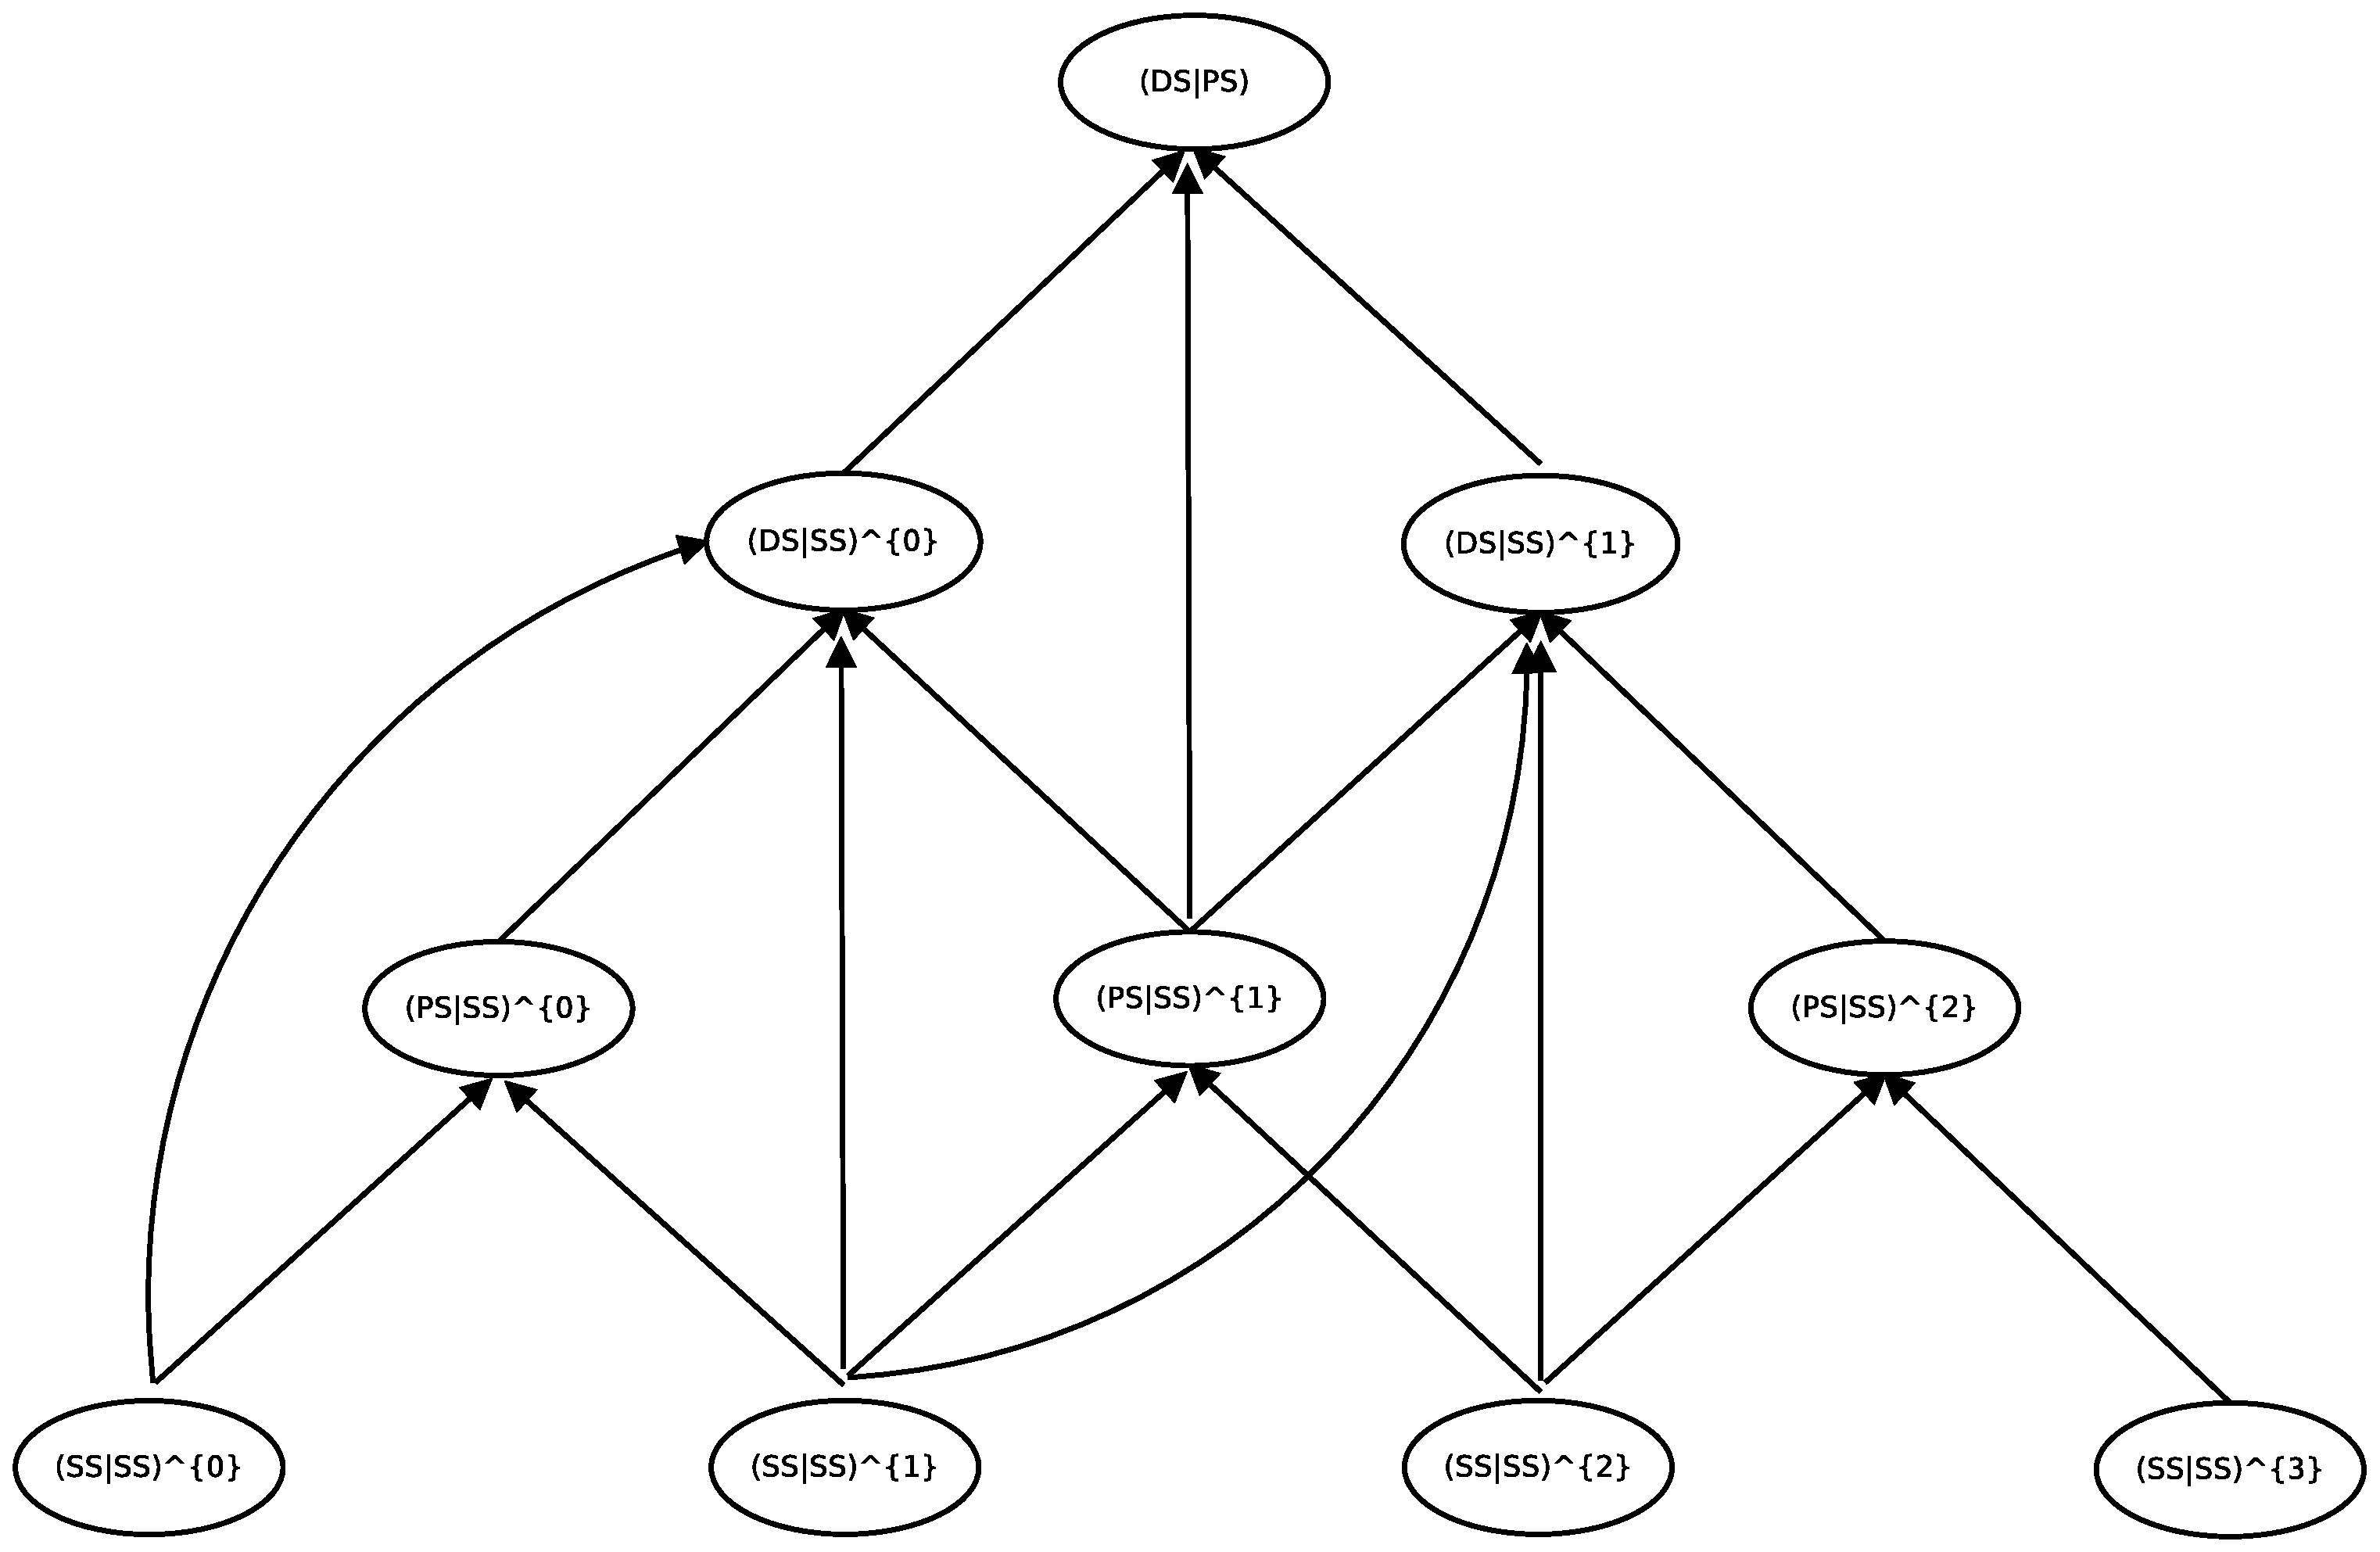
\includegraphics[scale=0.25]{./graph.eps}
 % general_rr.eps: 0x0 pixel, 300dpi, 0.00x0.00 cm, bb=0 0 763 487
 \caption{directed graph for integral of $(DS|PS)$ based on OS scheme}
 \label{fig:1}
\end{figure}

In CPPINTS, a general searching algorithm is used on solving the tree-search problem for 
VRR. Instead of exploring details for optimal path, by
investigating the nature of VRR formula we can wrap up correlated integrals into packages
and it turns out that the packages are independent with each other on the VRR path. Based on
the concept of package, the directed graph for VRR is converted into tree data structure and the optimal
path for VRR is corresponding to the shortest path in the given tree data structure, where the
a similar Dijkstra's algorithm\footnote{please see 
\url{http://en.wikipedia.org/wiki/Dijkstra\%27s_algorithm} for more information} is applied.
This part will be discussed in section \ref{optimal_path}.

For computing the target integrals, both VRR and HRR need many intermediate integrals on
the recurrence relation(RR) path. The interesting question is, is every intermediate integral 
necessary in the recurrence generation? The question becomes more interesting in terms of 
the redundancy of Cartesian type of Gaussian functions in comparison with the spherical form of 
Gaussian functions. In the section \ref{redundancy_rr} a general recursive procedure is 
employed to explore the redundancy of RR.


%%%%%%%%%%%%%%%%%%%%%%%%%%%%%%%%%%%%%%%%%%%%%%%%%%%%%%%
% optimal VRR path
%%%%%%%%%%%%%%%%%%%%%%%%%%%%%%%%%%%%%%%%%%%%%%%%%%%%%%%
\section{Finding Optimal Path for Recurrence Relation}
\label{optimal_path}

The optimal path for RR can be defined in variety of way. In this paper,
the optimal path is the implementation of RR with minimum intermediate integral
number. Our discussion below is based on HGP scheme above. However,the idea 
and implementation below is easy to transfer to other RR schemes.

In the practical implementation of RR, the integral calculation is usually performed 
in terms of shells rather than basis functions, so that to reduce the repeat use of 
intermediate integral. Considering the equation \ref{int_paper:3}, 
all of shell positions in the shell quartet $(FD|PS)$ are expandable except the ``ket2'' position 
where the shell is ``S'' type of 
function. Therefore for each LHS ERI appearing in the VRR, how to find it's proper expandable
position so that to minimize the total number of intermediate integrals is the key to 
find optimal path for VRR.

Let's take ERI as an example. The equation \ref{int_paper:3} can be generalized into a 8-term 
expansion:
\begin{align}\label{int_paper:7}
I(L,m) &= a_{0}I_{0}(L-1,m) + a_{1}I_{1}(L-1,m+1) \nonumber \\ 
&+ a_{2}I_{2}(L-2,m) - a_{3}I_{3}(L-2,m+1) \nonumber \\
&+ a_{4}I_{4}(L-2,m) - a_{5}I_{5}(L-2,m+1) \nonumber \\
&+ a_{6}I_{6}(L-2,m+1) + a_{7}I_{7}(L-2,m+1)
\end{align}
$L$ is the sum of angular momentum
\begin{equation}\label{int_paper:8}
 L = L_{a} + L_{b} + L_{c} + L_{d}
\end{equation}
for ERI $(ab|cd)$, and $m$ is the parameter for auxiliary integral $(ab|cd)^{(m)}$ in 
expression \ref{int_paper:4}.
From equation \ref{int_paper:7}, it's clear that the $L$ is constantly decreasing and $m$ is
increasing in same manner from LHS to RHS. Therefore the properties of $L$ and $m$ 
for ERI characterize an ``arrow'' in the derivation of VRR, in this sense the VRR
for ERI is ``inconvertible'' between LHS and RHS. As see in the following discussion,
such inconvertibility grantees the existence of conversion for transforming the graph
data structure into the tree data structure for ERI\footnote{In tree data structure,
every children node can only have one parent node. Such character establishes the direction
of the tree. Please see \url{http://en.wikipedia.org/wiki/Tree_\%28data_structure\%29} for 
more information}, and it also establishes an order 
of sequence between two arbitrary ERI so that RHS ERI is always generated prior to
the LHS ERI in the resulting VRR path.

Based on the feature of inconvertibility, it's able to set up some general coding structure
to perform the optimal path search for ERI in VRR (unsolved shell quartets are these who
appear in VRR path but their expanding position are not yet determined):
\begin{verbatim}
set up unsolved shell quartet archive;
initilize the unsolved shell quartet archive with 
input LHS shell quartets;
loop over m (from m=0 to maximum):
  loop over L (from maximum to 0):
    while(true):
      perform optimal expanding postion search for 
      all (L,m) LHS shell quartets in the unsolved 
      shell quartet archive;
      if there are no (L,m) LHS shell quartets break 
      out the loop;
    end while
  end loop with L
end loop with m
\end{verbatim}
The search is carried out from the LHS to RHS until all of LHS shell quartets 
are solved. The procedure here establishes a general Dijkstra algorithm scheme 
for searching expanding positions for VRR. By wrapping up all of unsolved 
$(L,m)$ shell quartets together, it's able to search their their optimal expansions
and the following search iteration will be performed based on the output of
previous iterations. 

How to evaluate the efficiency of the algorithm comparing with Breadth-first search
or Depth-first search across all of possible VRR paths? In general the Dijkstra algorithm
can not guarantee a global minimum because the global minimum may not be reached by
by assembling minimums on the partial path. However, because L is constantly decreasing
from LHS to RHS; the integral numbers are constantly decreasing from current search
iteration to the following ones. Therefore it could expect that the above procedure
may give the close VRR path comparing with the global optimum.

In terms of an arbitrary given unsolved $(L,m)$ shell quartets, all of shell quartets
appearing in VRR can be divided into three groups:
\begin{itemize}
 \item unsolved main list;
 \item correlated list;
 \item irrelevant list 
\end{itemize}
Unsolved main list contains the unsolved shell quartets with given properties of $(L,m)$.
Their expanding position are going to be determined in the current iteration of search. 
Correlated list is composed by the unsolved shell quartets who possibly share the RHS 
terms with the unsolved main list. The irrelevant list is composed by all of other 
unsolved shell quartets and their expansion positions are independent with the 
unsolved main list. By combining the unsolved main list and correlated list together 
to form a package, all of correlated LHS shell quartets are self-contained therefore 
it's able to carry out a full search on all possible expansion combinations for every 
LHS shell quartets inside the package. The search result gives the final expanding
positions to the unsolved main list.

Let's take ERI as illustration. The VRR in equation \ref{int_paper:7} demonstrates that 
for ERI $I(L,m)$, only ERI of $I(L-1,m)$, $I(L,m+1)$ and $I(L-1,m+1)$ can share RHS with it.
These ERI are in unsolved state and their undetermined expansion will affect the determination 
of expanding position for $I(L,m)$. On the other hand, although ERI with $L+1$ or $m-1$ are 
also possibly sharing RHS with $I(L,m)$, their expanding position have been solved in previous 
iteration; therefore these shell quartets apply deterministic effects on the search of expanding 
position searching for ERI $I(L,m)$. As a result of inconvertibility of VRR, the number of shell
quartets which constitutes the correlated package decreases significantly.

In summary, for searching the expanding position of shell quartets with property of $(L,m)$, 
it's able to form an independent package with unsolved shell quartets characterized by property 
$(L-1,m)$, $(L,m+1)$ and $(L-1,m+1)$. A complete survey to find minimum RHS integrals for $(L,m)$
shell quartets is performed in terms of all of possible expansion combinations for all of shell 
quartets inside the package. The implementation for the above algorithm is depicted as below:
\begin{verbatim}
set up archive for solved shell quartets;
set up archive for unsolved shell quartets;
initilize the unsolved archive with input shell quartets;

loop over m (from m=0 to maximum):
  loop over L (from maximum to 0):
    while(true)
      construct empty main shell quartet list, and fill 
      in shell quartets with (L,m) from unsolved archive;
    
      construct empty correlated shell quartet list, and 
      fill in possible shell quartets with (L-1,m), 
      (L,m+1) and (L-1,m+1) from unsolved archive;
      
      combine the main shell quartet list and appended
      shell quartet list together into full list;
      
      loop over all possible expanding combinations:
         compare the new RHS shell quartets with solved
         and unsolved archives, remove the new RHS shell
         quartet if it's double couting (vertical 
         comparison);
         
         compare the new RHS shell quartets with each 
         other and wipe out the repeat ones (horizontal
         comparison);
         
         count the number of integrals from all remaining 
         RHS shell quartets, replace the old expansion
         plan with new one if it's outperformed;
      end loop of expanding combination 
       
      for the optimal expansion plan, push the main
      shell quartets into solved archive and the new
      RHS shell quartets into unsolved archive;
       
      is there remaining shell quartets with property
      of (L,m) in unsolved archive?
      if not, step out the while loop;      
    end while
  end loop with L
end loop with m 
\end{verbatim}

The procedure establishes the result VRR path by assemble global minimum on each partial VRR
path along the searching iterations. Such pseudocode not only applies to ERI, but also to
KI, NAI etc. as long as the integral can be derived from recurrence relation with inconvertible
property. Unfortunately, HRR can not employ the above algorithm because the inconvertibility 
is destroyed inside HRR:
\begin{align}
\label{int_paper:9}
 (a(b+\iota_{i})|cd) &= ((a+\iota_{i})b|cd) + AB_{i}(ab|cd)   \nonumber \\
                     &\Updownarrow                            \nonumber \\
 ((a+\iota_{i})b|cd) &= (a(b+\iota_{i})|cd) - AB_{i}(ab|cd)   
\end{align}
For example, if LHS shell quartet $(FD|PS)$ is expanded in terms of shell D position according 
to equation \ref{int_paper:9}, in search of expanding position of result RHS shell quartet $(GP|PS)$
it will resort to the expansion on shell G because the previous LHS $(FD|PS)$ becomes the RHS for
expanding $(GP|PS)$ and $(FD|PS)$ is already contained in the result path. As a result, the expansion 
search forms a cycles and the expanding positions for LHS shell quartets are never to be correctly 
determined in the generated HRR path.

In HRR we use another way to determine the optimal path. Since HRR expansion only concentrates on
either bra or ket side, a trial expanding test is performed to determine the best bra/ket 
expansion for HRR. For ERI the trial expanding positions are grouped into four cases; namely 
as (bra1,ket1), (bra1,ket2), (bra2,ket1) and (bra2,ket2). For each position combination a HRR 
path searching is conducted and the final HRR path picks up the one which generates the minimum
integral number.

%%%%%%%%%%%%%%%%%%%%%%%%%%%%%%%%%%%%%%%%%%%%%%%%%%%%%%%
% application of rrsearch
%%%%%%%%%%%%%%%%%%%%%%%%%%%%%%%%%%%%%%%%%%%%%%%%%%%%%%%
\section{Application of Optimal Path for RR}

\subsection{Building RR Formula}
\label{rrbuild}
%
% this section introduce the RRbuild class
% 1  RR expanding position
% 2  RR formula for shell quartet
% 3  RR formula for integral
%
For constructing the recurrence relation, the first fundamental step is to set up some class
that we are able to describe the recurrence formula in the program. The class of RRbuild
is used to perform this job.

Generally, the formula of RR can be expressed as:
\begin{equation}\label{general_rr_formula}
 I_{LHS} = a_{0}I_{0} + a_{1}I_{1} + a_{2}I_{2} + a_{3}I_{3} + a_{4}I_{4} + \cdots
\end{equation}
All of $I_{i}$ is integral recursively derived from previous content. Usually the RHS
integrals or shell quartets in \ref{general_rr_formula} are formed by raising up or 
decreasing angular momentum or m value in terms of LHS. Sometimes the operator is also
changed from LHS to RHS, for example; the VRR expansion for two body kinetic integrals
in the OS framework.

A general RR formula has two properties. Firstly, for RR formula applying on
multiple body integrals the expanding position is needed to be specified. This is 
because there potentially has multiple expanding positions available for forming
the RR expansion on given integral or shell quartets\footnote{please refer to the 
discussion of \ref{optimal_path} for more details}, and usually different expanding 
position will lead to different result RR formula. For example, the HRR expansions
on ERI $(ab|cd)$ shown in equation \ref{int_paper:9} are different between expansion
on BRA1 and expansion on BRA2.

For RR expansion on shell quartets, if the RR algorithm and the expanding position
are both determined; then the RR formula is set up for the given shell quartet.
Under such circumstance, for the given LHS shell quartet it's able to derive
all of RHS shell quartets, and especially figure out which RHS shell quartet is 
``NULL''(it means this term does not appear in the result RR expansion). The function
of buildRRSQ in rrbuild.cpp is performing this work.

However, for the RR formula on integral the result RR formula is still unsolved yet.
With a determined expanding position on a given RR formula, to solve LHS integral
it's needed to specify the direction of RR formula. For example, the VRR expansion 
for ERI is:
\begin{equation}
 \begin{split}
((a+\iota_{i})b|cd)^{(m)} &= (P_{i} - A_{i})(ab|cd)^{(m)} +
\left(W_{i} -P_{i}\right)(ab|cd)^{(m+1)} \\
&+\frac{N_{i}(A)}{2\epsilon}\left(((a-\iota_{i})b|cd)^{(m)}-\frac{\rho}{
\epsilon }((a-\iota_{i})b|cd)^{(m+1)}\right)  \\
&+\frac{N_{i}(B)}{2\epsilon}\left((a(b-\iota_{i})|cd)^{(m)}-\frac{\rho}{
\epsilon }(a(b-\iota_{i})|cd)^{(m+1)}\right)  \\
&+\left(\frac{N_{i}(C)}{2}\right)\frac{1}{\epsilon+\eta}
(ab|(c-\iota_{i})d)^{(m+1)} \\
&+\left(\frac{N_{i}(D)}{2}\right)\frac{1}{\epsilon+\eta}
(ab|c(d-\iota_{i}))^{(m+1)}
\end{split}
\end{equation}
This expansion is on ``BRA1'' position. However, the direction information on $i$ 
could be x, y or z so that it needed to be specified. As long as the $i$ is specified,
it's able to derive the RHS integrals as well as the RHS coefficients like 
$PA_{i} = P_{i} - A_{i}$(i is x, y or z) or $N_{i}(A)$, $N_{i}(B)$ etc. appearing in
the formula \footnote{please refer to the code rrbuild.cpp or the original OS paper
\cite{OS1986} for the meaning of these symbols}.

The function of buildGeneralVRR and buildGeneralHRR are used to build a general 
RR formula in terms of a given position (position must be provided for RRBuild
class so that to construct a specific RR expansion). The function of determineDirection
is used to derive the undermined direction information for the given RR formula.
In fact, this is the core function for deriving the redundancy of RR(please see the 
section \ref{redundancy_rr} for more information). Because after
the direction is set, for the given LHS shell quartet it's able to figure out
what's the RHS integral is practically referred in the RR expansion. The unrefereed
integrals, or in other words; the unused integrals represent the redundancy of 
result RR path.

After direction of $i$ i set, accordingly it's able to figure out the $N_{i}$ value
appearing in the RR formula for the RHS integrals. This job is performed in function
determineNi of rrbuild.cpp. Finally, by bringing all of information together it's able
to derive the full RR formula for a given LHS integral from the function buildRRInt. 

\subsection{Optimal RR Path Search in RR}
\label{rrsqsearch}

The optimal RR path search is carried out in rrsqsearch.cpp. The implementation 
exactly follows the idea discussed in section \ref{optimal_path}.

The function RRSearchBasedOnTWOProperty in rrsqsearch.cpp realizes the pseudo codes
described in section \ref{optimal_path}. Considering VRR for different kinds of 
integrals, the VRR properties could be $L$ and $m$ (for example, ERI, NAI etc.);
or could be $L$ and operator type (two body kinetic integrals) etc. This function
performs optimal VRR path search based on two combined properties or one property
varied on VRR formula. 

The RRSQSearch class (which defined in the rrsqsearch) has two data members, one 
is solvedSQList, which stores the shell quartets which appears in the RR path and 
it' expanding position has been solved. The unsolvedSQArch stores all of undetermined
shell quartets so to keep as archive purpose during the path search.

As entering into the work loop in RRSearchBasedOnTWOProperty function, it sets up
two lists; one is unsolvedMainSQList which stores the result shell quartets for 
the corresponding properties (for example, for fixed $L$ and $m$), and the other
is unsolvedAppendSQList which is equivalent to the ``correlated shell quartet list'',
and it's used to store the correlated shell quartet list. In pickupUnsolvedSQ 
function, it forms both of two lists according to the discussion in section 
\ref{optimal_path}. Afterwards, the global search is performed in the function 
searchOptPos on both of the two lists, and the expanding positions will be determined
for the unsolvedMainSQList.

In rrsqsearch.cpp we set up another class, which is called RRShellQuart and it's 
used to hold all of it's possible expanding RR expansion information. In the 
searchOptPos, the input shell quartet list will be transfered into a list of 
RRShellQuart so that it contains all of possible expansion information. Finally,
by setting up a multi-dimensional array whose name is loop\_identifier(see the 
comments of the code), we loop over all of possible combinations between the 
expanding position for each input shell quartet; and finally derive the position
where minimum number of integrals are generated.

%%%%%%%%%%%%%%%%%%%%%%%%%%%%%%%%%%%%%%%%%%%%%%%%%%%%%%%
% redundancy
%%%%%%%%%%%%%%%%%%%%%%%%%%%%%%%%%%%%%%%%%%%%%%%%%%%%%%%
\section{Redundancy Analysis for RR}
\label{redundancy_rr}

After the optimal VRR/HRR path is set, the next step is to generate 
the recursive expansion on integrals for each shell quartet on the 
path so to complete the forming of RR. The integral
generation implicitly comes with a question, is every integrals in 
the shell quartet needed by the RR? This open question becomes more 
interesting considering the natural redundancy inside the Cartesian 
type of Gaussian functions comparing with the spherical type of Gaussian
functions.

The answer for this question is varying from case to case, therefore there's 
no general estimation can be made and the problem need to be investigated 
on the fly. For studying the redundancy of integral inside RR, we propose
a general algorithm to generate integrals for the a given RR path:
\begin{verbatim}
set up LHS list and initialize it
with input shell quartets;
set up result RR formula archive;
while(true):
  loop over the LHS shell quartets in the LHS list:
    form RR formula on integrals for the given LHS 
    shell quartet;
    if the LHS not appear in RR path, push the new 
    RR formula into archive and exact the RHS 
    information;
    else merge the new RR formula with the old one
    which already appears in the archive;
  end loop
  do we have any new RHS terms? if not, exit the loop;
  exacting all of new RHS terms and form new LHS list;
end while
\end{verbatim}
For some shell quartets the above procedure can not grantee that every
RHS integrals are defined previously. For solving the incompleteness,
a similar code like above is performed for all of missing RHS integrals
to ensure the completeness of RR. We implemented the procedures for 
both VRR and HRR.
 
%%%%%%%%%%%%%%%%%%%%%%%%%%%%%%%%%%%%%%%%%%%%%%%%%%%%%%%
% how to realize RR
%%%%%%%%%%%%%%%%%%%%%%%%%%%%%%%%%%%%%%%%%%%%%%%%%%%%%%% 
\section{RR Formulation}

\subsection{Building RR Expression for Each Shell Quartet}
%
%  1  what is unsolved integral list
%  2  whether it's integal index or not?
%  3
%
%
For each LHS shell quartet on the RR path, to build explicit RR expression
the following information are needed:
\begin{itemize}
 \item the expanding position which is derived from RRSQSearch class in 
 \ref{rrsqsearch};
 \item general RR expanding formula set up by RRBuild class in \ref{rrbuild};
 \item the unsolved integral list corresponding to the LHS shell quartet 
\end{itemize}
Unsolved integral list contains all of LHS integrals. We only form RR expansion
for the given integral list, and it implies that the integral list could be 
only a subset of the whole integrals corresponding to the LHS shell quartet.
This is the natural result deriving from the redundancy of using Cartesian
form of basis set function in RR (see section \ref{redundancy_rr} for more
details). Unsolved integral list is generated during the RR process from
the RHS shell quartet in the subsequent context (the generation of unsolved
integral list is referred to section \ref{rr_code}).

In the previous section \ref{mapping_integral_sq}, we stated that
in the RR formation the integrals is actually expressed by it's index
in the corresponding shell quartet. Here the unsolved integral list
is also formed as index list. During the whole RR process all of integrals
on both RHS and LHS are all referred as index form. After the RR is formed,
however the original index could be destroyed and replaced with ``array index''.

The array index refers to the final position of the integral in the result
code. For example, $(DD|PP)$ has 324 integrals in total, however in the RR
process it only uses 270 integrals so there are 54 unused integrals appear
as redundancy. The integral index forms the one to one mapping between  
the integral itself and the shell quartet, the array index characters the 
final position for the given integral, for example; the position index of 
$(D_{xy}D_{yz}|P_{x}P_{z})$ in SQ\_DDPP array in the result code. If the 
integral index is transformed into array index, all of index information
can not be restored (see the comment in rrints.h for more details). This 
is what function rhsArrayIndexTransform and lhsArrayIndexTransform do.

for a given specific unsolved integral list, RRInts may create it's RR 
expression if this is a fresh new LHS shell quartet on the RR path, this
is done through the constructor; or do updating if the given LHS shell 
quartet already exists. The updating function is performed in function
updateLHS. This function will search the new integral from the input
unsolved integral list and merge it's RR expression into the current RR
expression archive. This is the core function to perform ``completeness
check'' step described in \ref{redundancy_rr} and \ref{rr_code}.

\subsection{Forming RR Path}
\label{rr_code}
%
% 1  the general steps to form RR
% 2  what's the purpose rrsqsearch?
% 3  how to create all of rrsq information?
% 4  how to do updating function
% 5  sorting function of RR
%
Based on the rrints.cpp, now we are able to form whole RR path for 
either VRR or HRR. Generally RR formation requires the following 
steps:
\begin{itemize}
 \item for the input shell quartet list(they are the results of RR path), 
 finds all of shell quartets on the RR path through RRSQSearch class;
 \item derive the initial unsolved integral list from the input 
 shell quartets, building RR for each LHS shell quartet recursively
 until the RR path reaches it's top;
 \item sorting the whole RR so that to establish the direction from
 LHS to RHS or RHS to LHS;
 \item completeness check to see whether we have undefined LHS integrals.
 If so, rrUpdating function is called to complement RR path;
 \item transform all of integral index into array index if the given RR
 section only uses array in printing the code
\end{itemize}

As the initial step, RRSQSearch class finds all of shell quartets appearing
in the optimum RR path by the giving input shell quartet list. Additionally,
it also determines the RR expanding position for each shell quartet. 

After the shell quartet is set, function of formRRSQList begins to build 
the whole RR content. By calling function buildRRSQList iteratively, 
formRRSQList form RR details for each bunch of LHS shell quartets and it's 
unsolved integral list. The pseudo code for buildRRSQList is like this:
\begin{verbatim}
set up initial LHS shell quartet list and initialize 
the corresponding unsolved integral list;
while(true):  
  Have all of the LHS shell quartets been built in
  the existing RR path? Or the LHS shell quartets
  are bottom integrals? If so, break;
  For the new LHS shell quartet, build it's RR 
  through RRSQ class in rrints.cpp and push it
  into the RR path;
  Get the RHS shell quartets (unsolved ones) and 
  it's corresponding unsolved integral list from
  RRSQ, and replace the LHS shell quartet and 
  the unsolved integral list with the new content
end while 
\end{verbatim}

As we stated early in section \ref{redundancy_rr}, during 
this process it's possible that some LHS integral may 
not be defined; therefore the ``completeness check''
step is needed to be performed in function of completenessCheck.
After identifying the missing undefined LHS integrals
the function of rrUpdating will complete the definition
for all of LHS integrals in RR.

For either HRR or VRR, one of necessary function is to sort
the result RR path so that to print the RR exactly from 
LHS to RHS. The core of sorting function is embedded in the 
shell quartet class (see \ref{sort_shell_quartet} for more 
details), and RRSQ class in rrints.cpp set up the operator
$<$ by using the core function in shell quartet class.

%%%%%%%%%%%%%%%%%%%%%%%%%%%%%%%%%%%%%%%%%%%%%%%%%%%%%%%%%%%%%%%%%%%%%%%%
\section{Top Level Classes of CPPINTS}

In this section, we will discuss the working classes on the top of 
the working modules of RR, so as to complete the whole integrals
forming.

%%%%%%%%%%%%%%%%%%%%%%%%%%%%%%%%%%%%%%%%%%%%%%%%%%%%%%%
% infor class
%%%%%%%%%%%%%%%%%%%%%%%%%%%%%%%%%%%%%%%%%%%%%%%%%%%%%%%
\subsection{Gathering Input Information from User}
\label{infor_class}

infor.cpp establishes an communication between the user and CPPINTS
program. In the Infor class, CPPINTS allows the user to manipulate
the generation of integrals through user-specified options which is 
defined in parameter file. All of options that user can access is 
explained in detail through a sample file named as ``infor.txt''. 

%%%%%%%%%%%%%%%%%%%%%%%%%%%%%%%%%%%%%%%%%%%%%%%%%%%%%%%
% sqints
%%%%%%%%%%%%%%%%%%%%%%%%%%%%%%%%%%%%%%%%%%%%%%%%%%%%%%%
\subsection{SQInts class: Deriver of RR formation}

Based on all of the working classes described above, now it's capable of 
generating the analytical integral based on RR formula.

In general, the analytical integral code can be divided into following 
sections in terms of VRR and HRR:
\begin{itemize}
 \item VRR step:
 \begin{itemize}
    \item set up VRR results in either variable form or array form, VRR 
    results are also the input of HRR step;
    \item step into VRR loop, prepare VRR variables;
    \item calculate the bottom integrals for VRR;
    \item print out whole VRR until the result integrals are generated;
    \item contraction the result with possible coefficients or other 
    variables
 \end{itemize}
\item HRR step:
 \begin{itemize}
    \item prepare the HRR variables;
    \item do HRR for the first side (bra or ket) so to generate HRR results
    from the VRR results;
    \item if second side HRR is necessary, then to generate HRR results 
    from the results on first side;
    \item generate the final results
 \end{itemize}
\end{itemize}

SQInts class is the deriver function to perform the integral generation based
on the above scheme. Generally SQInts generates the temporary integral file 
in the reverse order, that is from HRR second side(file with .hrr2), to HRR 
first side(file with .hrr1), then to VRR(file with .vrr); then SQInts 
assembles all of parts together into a complete integral code file.

The function of doHRR performs the two steps HRR work together. Each step of HRR 
work is performed through doCoreHRR function. The functions also determines that 
whether the HRR work on the given side is not needed. VRR work is carried out 
in the doVRR function.

There are a lot of details corresponding to the code generation. To make the 
code more clearer, we separate the printing functions, as well as the information
generation functions outside the SQInts class and form SQIntsInfor and SQIntsPrint
classes instead. Therefore, SQInts is able to become a clear, and thin driver
class on top of all of working classes including SQIntsInfor and SQIntsPrint.

%%%%%%%%%%%%%%%%%%%%%%%%%%%%%%%%%%%%%%%%%%%%%%%%%%%%%%%
% sqintsinfor
%%%%%%%%%%%%%%%%%%%%%%%%%%%%%%%%%%%%%%%%%%%%%%%%%%%%%%%
\subsection{SQIntsInfor class}

SQIntsInfor is designed for holding the fundamental information for RR process
in terms of input shell quartets. The idea is to wrap up these information into
an object, then it's easy to deliver it to different places whenever it's needed;
for example, into RR object etc.

The information contained in the SQIntsInfor is formed in terms of the input
shell quartets, it includes:
\begin{itemize}
 \item variable form (array or single variable) for VRR and HRR;
 \item whether it do file split because code is too large;
 \item HRR first side and second side;
 \item job order;
 \item operator information;
 \item input shell quartets (here the composite shell quartets will
 be decomposed into pure ones);
 \item  offset information
\end{itemize}


%%%%%%%%%%%%%%%%%%%%%%%%%%%%%%%%%%%%%%%%%%%%%%%%%%%%%%%
% sqintsprint
%%%%%%%%%%%%%%%%%%%%%%%%%%%%%%%%%%%%%%%%%%%%%%%%%%%%%%%
\subsection{SQIntsPrint class}
 
In the process of generating the result integral code, there are a lot of 
additional parts need to be printed besides the RR codes. For example,
produce the function name and it's parameters; prepare the VRR variables
as well as bottom integrals for VRR and HRR etc. All of these printing 
requirements are folded into one sophisticated class SQIntsPrint, this 
class is primarily a collection of different functions in terms of 
printing purpose. 

%%%%%%%%%%%%%%%%%%%%%%%%%%%%%%%%%%%%%%%%%%%%%%%%%%%%%%%
% fmt
%%%%%%%%%%%%%%%%%%%%%%%%%%%%%%%%%%%%%%%%%%%%%%%%%%%%%%%
\subsection{A New Scheme for calculating $f_{m}(t)$}
\label{fmt}

The $f_{m}(t)$ integral
\begin{equation}\label{fm_ssssm_fmt_eq:1}
 f_{m}(t) = \int^{1}_{0} u^{2m} e^{-tu^{2}} du 
\end{equation}
is a necessary component in calculating the bottom integrals of ERI $(00|00)^{m}$,
NAI $(0|0)^{m}$ etc. Its calculation has been discussed in details in literature
\cite{harris1983sssm, gill1991two} etc. Here we try to present our model to calculate
$f_{m}(t)$ in terms of a hybrid scheme, the implementation of the scheme can be 
found in fmtIntegralsGeneration function of SQIntsPrint class.

As $m=0$ the $f_{m}(t)$ becomes error function:
\begin{equation}
 f_{0}(t) = t^{-\frac{1}{2}} erf(t^{\frac{1}{2}})
\label{fm_ssssm_fmt_eq:2}
\end{equation}
which is available in variety of standard libraries. For $m>0$, $f_{m}(t)$
is incomplete Gamma function and it satisfies a recursive expression:
\begin{equation}
  f_{m}(t) = \frac{1}{2m+1}\left( 2tf_{m+1}(t) + e^{-t}\right)  
 \label{fm_ssssm_fmt_eq:3}
\end{equation}
thus $f_{m}(t)$ can be derived from $f_{m_{max}}(t)$. On the other hand, equation
\ref{fm_ssssm_fmt_eq:3} can be reorganized as:
\begin{equation}
  f_{m}(t) = \frac{1}{2t}\left( (2m-1)f_{m-1}(t) - e^{-t}\right)    
 \label{fm_ssssm_fmt_eq:4}
\end{equation}
This expression provides the easiest way to compute the $f_{m}(t)$ by starting from 
$f_{0}(t)$. However, equation \ref{fm_ssssm_fmt_eq:4} is numerically instable due to
error propagation as $m$ grows larger.

$f_{m}(t)$ is able to be expanded as polynomial series:
\begin{equation}
 \label{fm_ssssm_fmt_eq:5}
 f_{m}(t) = e^{-t}\sum_{k=0}^{\infty}\frac{(2m-1)!!}{(2m+2k+1)!!}
 (2t)^{k}
\end{equation}
The problem for equation \ref{fm_ssssm_fmt_eq:5} is that it converges very slow as $t$
grows larger, therefore this expression is typically used for small t. As $t$ becomes large,
a continued fraction representation can be used to compute $f_{m}(t)$\cite{harris1983sssm}:
\begin{equation}
\begin{split}
f_{m}(t) &= \frac{(2m-1)!!\sqrt{\pi}v^{m}}{2t^{\frac{1}{2}}} \\
         &- e^{-t}
         \left\lbrace 
         \frac{v}{1+}\frac{(1-2m)v}{1+}\frac{2v}{1+}\frac{(3-2m)v}{1+}\frac{4v}{1+}
         \frac{(5-2m)v}{1+}\frac{6v}{1+\cdots}
         \right\rbrace 
\end{split}
\label{fm_ssssm_fmt_eq:6}
\end{equation}
where $v = (2t)^{-1}$. Although equation \ref{fm_ssssm_fmt_eq:6} can yield very accurate
result, it's implementation is inefficient comparing with equation \ref{fm_ssssm_fmt_eq:4}.

Many standard libraries adopt the hybrid strategy for implementing $f_{m}(t)$. For instance,
BOOST library\footnote{please see \url{http://www.boost.org/} for more details} expands 
$f_{m}(t)$ into polynomial series for small $t$, for large $t$ it uses
Legendre's continued fraction representation for computation. However, is it possible 
to find a range in terms of $t$ and $m$ that $f_{m}(t)$ can be accurately calculated from
equation \ref{fm_ssssm_fmt_eq:4} so that to avoid the use of continued fraction representation?

As $t$ is small it's applicable to employ the polynomial expression of \ref{fm_ssssm_fmt_eq:5} to 
accurately compute $f_{m}(t)$ for variety of $m$, hence the problem concentrates on how to calculate 
$f_{m}(t)$ for large $t$. Because equation \ref{fm_ssssm_fmt_eq:4} will yields larger error as $m$ grows, 
we try to find a limit of $m$; where under the limit it's able to use recurrence relation
\ref{fm_ssssm_fmt_eq:4} to compute $f_{m}(t)$ when $t$ is large, and above the limit the recurrence 
relation \ref{fm_ssssm_fmt_eq:3} is applied together with the calculation of $f_{m_{\max}}(t)$. This 
hybrid procedure can be summarized as:
\begin{enumerate}
 \item if $M_{max} == 0$, use error function;
 \item if $M_{max} >= 1$ and $M_{max} <= M_{limit}$:
 \begin{enumerate}
  \item if $t<=T_{limit}$, calculate $f_{M_{max}}(t)$ by using polynomial expansion of 
  \ref{fm_ssssm_fmt_eq:5}, then use recurrence relation \ref{fm_ssssm_fmt_eq:3} to compute 
  the rest of $f_{m}(t)$;
  \item if $t>T_{limit}$, calculate $f_{0}(t)$ with error function and 
  use recurrence relation \ref{fm_ssssm_fmt_eq:4} to derive other $f_{m}(t)$;
  \end{enumerate}
 \item if $M_{max} > M_{limit}$:
  \begin{enumerate}
     \item if $t<=T_{limit}$, calculate $f_{M_{max}}(t)$ by using polynomial expansion of 
  \ref{fm_ssssm_fmt_eq:5}, then use recurrence relation \ref{fm_ssssm_fmt_eq:3} to compute 
  the rest of $f_{m}(t)$;
   \item  if $t>T_{limit}$, calculate $f_{M_{max}}(t)$ 
  and use recurrence relation in \ref{fm_ssssm_fmt_eq:3} for all of other $f_{m}(t)$.
  \end{enumerate}
 \end{enumerate}
$M_{max}$ is the largest $m$ value for $(00|00)^{m}$ type of integrals, $T_{limit}$
represents the maximum limit of $t$ used in polynomial expansion \ref{fm_ssssm_fmt_eq:5};
and $M_{limit}$ is the limit of $m$ value that recurrence relation \ref{fm_ssssm_fmt_eq:4}
is able to be applied.

To explore the best $T_{limit}$ and $M_{limit}$ combinations, a trial test is performed on
the above hybrid scheme\footnote{Please see section \ref{use_util_codes}. The fmt\_test
in the util folder stores the testing code and comparison result log files}. 
In this test the $T$ value is sampled in step length of 1.0E-6
between $0$ and $T_{limit}$ for equation \ref{fm_ssssm_fmt_eq:5}, and recurrence relation 
\ref{fm_ssssm_fmt_eq:4} employs $T$ from $T_{limit}$ to $T_{max}$ with same step length.
When $T$ is large enough, the $e^{-t}$ term in equation \ref{fm_ssssm_fmt_eq:4} 
becomes 0 thereafter the recurrence relation becomes stable in terms of error propagation.
Considering this fact the $T_{max}$ is set to be $40.0$. For polynomial expansion 
\ref{fm_ssssm_fmt_eq:5}, $m$ is tested between $0$ and $40$. All of trial tests use 
the BOOST library for calculating the standard $f_{m}(t)$.

In the trial test the polynomial expression \ref{fm_ssssm_fmt_eq:5} 
always keeps maximum absolute error within 1.0E-14 for the given $T_{limit}$, and the 
maximum absolute error(MAE) for recurrence relation \ref{fm_ssssm_fmt_eq:4} with regarding to 
different $T_{limit}$ and $M_{limit}$ combinations is shown in table \ref{table:1}. 
It can be found that the all of MAE is below 1.0E-12, and 
with $T_{limit}=2.0$, $M_{limit}=8$ recurrence relation \ref{fm_ssssm_fmt_eq:4} reports
MAE of 1.0E-14; thus it can be well expected the hybrid scheme is able to generate satisfiable
accuracy for most of applications.

\begin{table}
\caption{maximum absolute error for recurrence relation \ref{fm_ssssm_fmt_eq:4}}
\label{table:1}
\begin{center}
\begin{threeparttable}
\begin{tabular}{c|c|c|c}
\hline
                    &       M = 8         &      M = 9        &   M = 10          \\
\hline
T = 1.8(18 terms)\tnote{a}   
                    &       3.0E-14       &      1.2E-13      &   6.3E-13         \\
\hline
T = 1.9(20 terms)   &       2.0E-14       &      0.7E-13      &   3.4E-13         \\
\hline
T = 2.0(22 terms)   &       1.0E-14       &      0.4E-13      &   2.0E-13         \\
\hline
\end{tabular}
\begin{tablenotes}
    \item[a] this is the No. of terms used in equation \ref{fm_ssssm_fmt_eq:5}
\end{tablenotes}
\end{threeparttable}
\end{center}
\end{table} 


